%% LyX 2.2.2 created this file.  For more info, see http://www.lyx.org/.
%% Do not edit unless you really know what you are doing.
\documentclass[english]{scrartcl}
\usepackage[T1]{fontenc}
\usepackage[latin9]{inputenc}
\usepackage{geometry}
\geometry{verbose,tmargin=2cm,bmargin=2cm,lmargin=3cm,rmargin=3cm,headheight=1cm,headsep=1cm,footskip=1cm}
\usepackage{babel}
\usepackage{calc}
\usepackage{graphicx}
\usepackage[unicode=true,pdfusetitle,
 bookmarks=true,bookmarksnumbered=false,bookmarksopen=false,
 breaklinks=false,pdfborder={0 0 1},backref=false,colorlinks=false]
 {hyperref}
\usepackage{breakurl}

\makeatletter
%%%%%%%%%%%%%%%%%%%%%%%%%%%%%% User specified LaTeX commands.
\usepackage{tikz}
\usepackage{changepage}
\usepackage{listings}
\addtokomafont{disposition}{\rmfamily}
\addtokomafont{descriptionlabel}{\ttfamily}
\usetikzlibrary{shapes.geometric}

% Definitions for XML syntax highlighting.
\definecolor{maroon}{rgb}{0.5,0,0}
\definecolor{darkgreen}{rgb}{0,0.5,0}
\lstdefinelanguage{XML}
{
basicstyle=\ttfamily,
morestring=[s]{"}{"},
morecomment=[s]{?}{?},
morecomment=[s]{!--}{--},
commentstyle=\color{darkgreen},
moredelim=[s][\color{black}]{>}{<},
moredelim=[s][\color{red}]{\ }{=},
stringstyle=\color{blue},
identifierstyle=\color{maroon}
}

\makeatother

\usepackage{listings}

\usepackage{float}
\usepackage{caption}
\newfloat{Annotation}{htbp}{loa}

\begin{document}

\title{Goal Manager Documentation}

\author{Luca Brusatin}

\date{\today}
\maketitle
\begin{abstract}
The Goal Manager (also called the Action Manager or simply ``Action'')
manages and executes agents' tasks (goals) in ADE. In addition to
simple action execution, the Goal Manager keeps track of the agents'
state (using the Belief Component) and verifies that all goals and
actions are acceptable and that the conditions for their execution
are met. When interfaced with a Planner Component\footnote{TODO: Currently the (RPI) planner is integrated within Action},
the Goal Manager can plan as well as avoid and resolve conflicting
actions.
\end{abstract}
\tableofcontents{}

\pagebreak{}

\section{Using the Goal Manager}

\subsection{Building, testing and launching the Goal Manager}

The Goal Manager component can be built with the \texttt{action}. The
tests action be built with the \texttt{action-test} target.

\subsection{Arguments\label{subsec:Arguments}}

The Goal Manager requires/supports the following arguments: 
\begin{description}
\item [{-agentname~{[}name{]}}] (optional, default: self)\\
Specifies the name of the agent for which the Goal Manager is responsible.
The Goal Manager will default to this name if no specific agent name
is provided during the execution of an action (\texttt{?actor} variable).
Sometimes referred to as ``super agent name'' in multi-agent settings.
\item [{-badaction~{[}name{]}}] (optional, repeatable)\\
Forbids the Goal Manager from using this action.
\item [{-badstate~{[}predicate{]}}] (optional, repeatable)\\
Forbids the Goal Manager from ending up in a state described by the
predicate.
\item [{-belief}] (optional)\\
Register for Belief Component notifications.
\item [{-beliefargs~{[}args{]}}] (optional)\\
Arguments to provide to the Belief Component instances spawned by
the Goal Manager.
\item [{-beliefcomponent}] (optional)\\
Specifies the name of the Belief Component to be used by the Goal
Manager for the first (``main''/''real'') state machine. If this
argument is used, the associated Belief Component has to be manually
started.
\item [{-dbfile~{[}path{]}}] (optional, repeatable)\\
Loads the contests of the file into the Action Database.
\item [{-selector~{[}class{]}}] (optional, default: \texttt{com.action.selector.UtilitarianActionSelector})\\
Uses the specified Action Selector mechanism to choose the best action
to execute.
\item [{-editor}] (optional)\\
Shows the Goal Manager GUI. Shows the contents of the Action Database
and provides a script editor.
\item [{-goal~{[}predicate{]}}] (optional, repeatable)\\
Executes the specified goal as an initial goal.
\end{description}

\subsection{Interfacing with the Goal Manager}

The Goal Manager interface provides a set of methods that allow other
ADE components to submit goals and query for the currently running
goals and their status. See \texttt{com/action/GoalManager.java}

\subsection{Goal Manager GUI/Editor}

The GoalManager GUI (figure \ref{fig:Goal-Manager-GUI/Editor.}) has
functionality for exporting existing entries to new files, deleting
entries, adding, duplicating, editing, and saving ActionDBEntries.

\medskip{}

In order to run the GUI, run the and the Goal Manager:

\noindent\begin{minipage}[t]{1\columnwidth}%
\begin{center}
\texttt{ant launch -Dmain=com.action.GoalManagerComponent -Dargs=\textquotedbl{}-editor\textquotedbl{}}
\par\end{center}%
\end{minipage}

\medskip{}

\begin{figure}
\begin{centering}
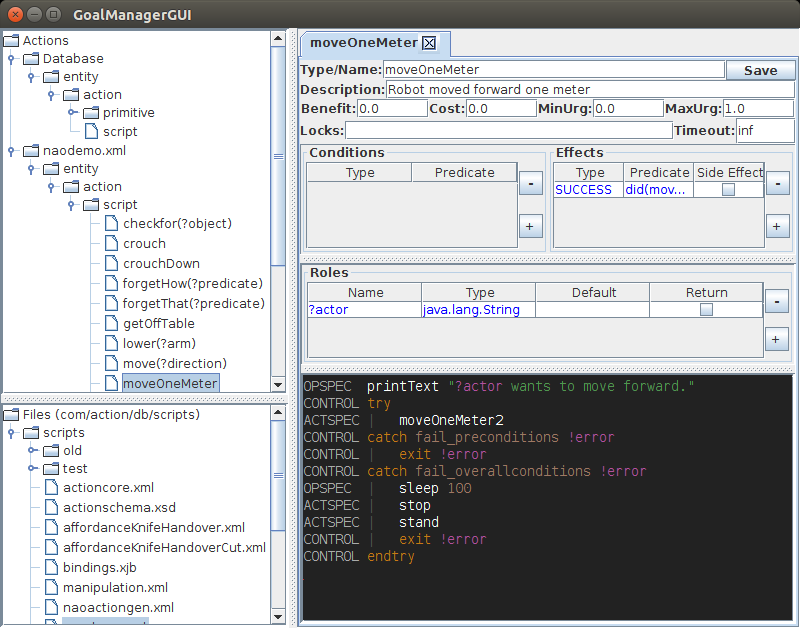
\includegraphics[width=0.8\columnwidth]{figures/editor}
\par\end{centering}
\caption{\label{fig:Goal-Manager-GUI/Editor.}Goal Manager GUI/Editor. The
editor has access to the Action Database and shows the available actions
in the top-left tree view. The bottom-left tree view shows the available
actions scripts. Double-clicking a file loads it into the editor and
the file appears in the top-left tree view, where nodes can be expanded.
Double-clicking on an action opens the script editor (right). Context
menus (right-click) provide additional functionality, such as loading
a script file into the Action Database, or removing an action from
the Database.}

\end{figure}


\section{Understanding the Goal Manager}

\subsection{Goals}

Goals are described by DIARC first order logic (FOL) predicates. They represent a desired state
that the Goal Manager has to achieve using the actions available to
it. Goals are sometimes called ``post-conditions''. If multiple
actions can achieve the same goal, the Goal Manager will choose one
using the Action Selector mechanism.

\medskip{}

A central principle in Goal Manager is the execution of goals, not
``actions''. By this, we mean that it is the end effect that we're
interested in, not the specific implementation of the action. Instead
of telling the robot to \texttt{moveTo X}, we'd rather have the robot
be \texttt{at(X)}. Let's expand our \texttt{moveTo} example a little
bit to explain things. Say the robot has a \texttt{moveTo} action
that requires the robot to be at a specific starting location for
it to work. Now let's say the robot also has another \texttt{moveTo}
action that does not require a specific starting location, but would
for instance be slower to execute. Both actions result in \texttt{at(X)}.
By submitting a task through a goal specification, e.g. \texttt{at(home)},
we give the Goal Manager the freedom to choose the most appropriate
action to fulfill this goal. It would, in this case, look up actions
that result in at(\texttt{X}) and, for each action, check if it is
permissible. If the starting location condition of \texttt{moveTo}
is met, the Goal Manager would have the choice between both \texttt{moveTo}
implementation and \textendash{} if the Action Selector is setup appropriately
\textendash{} choose the faster one. If now the starting location
condition is not met, the Goal Manager would choose the slower but
more generic \texttt{moveTo} action.

\subsubsection{\label{subsec:Post-conditions}Post-conditions}

A post-condition is a predicate that represents an effect of an action. 
The term ``post-condition'' is used because we would like to check that 
the execution of an action actually resulted in the \textbf{intended} 
effect; it is a condition necessary for the success of an action. 
Currently, post-conditions are only checked if they are observable
(i.e. an observer exists for the predicate). Otherwise the effects are 
just assumed to hold.

\subsubsection{\label{subsec:Generic-post-conditions} Submitting goals by action signature}

As explained prevously, actions are executed when a corresponding
goal is submitted to the Goal Manager. Sometimes we would like to
be able to ``call'' an action by name, generally because we do not
have a post-condition. This is the case for instance when a goal is
submitted through speech input (Dialogue), where the user input might
be ``walk forward''. Before the use of generic post-conditions,
we would translate ``walk forward'' to ``walking forward'' or
``walked forward'' which would be the post-condition of an action.
This required manual coding of the present progressive or past tense
for each action submitted through Dialogue. To avoid this, we allow
goals to be action signatures as well as post-conditions.

This used to be handled by auto-generating generic post-conditions for
every action, but this is no longer how the Goal Manage handles
this case. The Goal Manager now automatically detects if a goal
is a post-condition or an action signature.


\subsubsection{Goal submission}

As explained above, goals \textendash{} described by predicates \textendash{}
are submitted to the Goal Manager for execution. Figure \ref{fig:Goal-sumission-process.}
describes the goal submission process. Note that the execution of
actions associated with a Goal happens in a separate thread (ActionInterpreter).
Goals can therefore be executed simultaneously, in parallel.

\begin{figure}
\begin{center}
	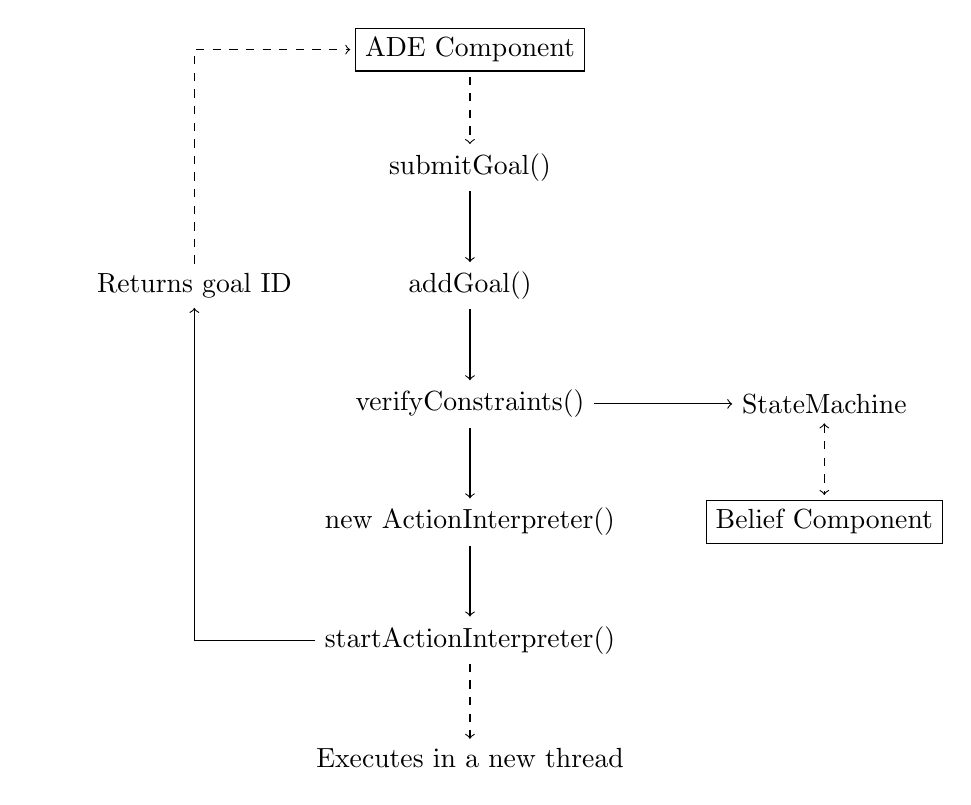
\begin{tikzpicture}[node distance=1.5cm,every node/.style={fill=white},align=center]
	% Specification of nodes (position, etc.)
	\node (start)				[draw, outer sep=2pt]	{ADE Component};
	\node (submitGoal)	[below of=start]						{submitGoal()};
	\node (addGoal)			[below of=submitGoal]				{addGoal()};
	\node (verifyCstr)	[below of=addGoal]   				{verifyConstraints()};
	\node (stateMachine)[right of=verifyCstr, xshift=3cm]
																									{StateMachine};
	\node (belief)			[below of=stateMachine, draw, outer sep=2pt]
																									{Belief Component};
	\node (newAI)				[below of=verifyCstr]  			{new ActionInterpreter()};
	\node (startAI)			[below of=newAI]						{startActionInterpreter()};
	\node (runAI)				[below of=startAI]					{Executes in a new thread};
	\node (return)			[left of=addGoal, xshift=-2cm, text width=4cm]	
																									{Returns goal ID};

	% Specification of lines between nodes specified above
	% with aditional nodes for description 
	\draw[dashed, ->]		(start) -- (submitGoal);
	\draw[->]						(submitGoal) -- (addGoal);
	\draw[->]						(addGoal) -- (verifyCstr);
	\draw[->]						(verifyCstr) -- (stateMachine);
	\draw[dashed, <->]	(stateMachine) -- (belief);
	\draw[->]						(verifyCstr) -- (newAI);
	\draw[->]						(newAI) -- (startAI);
	\draw[->]						(startAI) -| (return);
	\draw[dashed, ->]		(return) |- (start);
	\draw[dashed, ->]		(startAI) -- (runAI);
	\end{tikzpicture}
\end{center}

\caption{Goal sumission process.\label{fig:Goal-sumission-process.}}

\end{figure}


\subsubsection{Goal status}

Using the getGoalStatus() method, DIARC Components can query the state
of the execution of a goal. The following states are defined:
\begin{description}
\item [{UNKNOWN}] when a goal is not found
\item [{PENDING}] submitted but not yet being executed
\item [{ACTIVE}] execution of goal is in progress
\item [{SUSPENDED}] execution of goal has been suspended
\item [{CANCELED}] execution of goal has been cancelled
\item [{SUCCEEDED}] goal executed successfully
\item [{FAILED}] execution failed
\end{description}

\subsection{Actions\label{subsec:Actions}}

Actions can be defined in two different ways, as ``primitives''
or ``scripts''. An action primitive is nothing more than a Java
method annotated with the \texttt{@Action} (and \texttt{@TRADEService})
annotation (directly in the java interface). An action script is an
ASL (action script language) file describing a sequence of instructions which can be actions
(primitives or scripts), operators (e.g +, \texttt{-}, ...) or control-flow
elements (\texttt{if}, \texttt{while}, ...).

\subsubsection{Action status}

Actions are executed as steps towards achieving a desired goal state.
Using the getActionStatus() method, DIARC Components can query the state
of the execution of an action (which is being executed as part of some goal). The following states are defined:
\begin{description}
\item [{UNKNOWN}] when an action is not found
\item [{INITIALIZED}] execution of the action just started
\item [{APPROVED}] execution of action is approved
\item [{PROGRESS}] execution of action is in progress
\item [{VERIFYING\_EFFECTS}] observable effects are being verified
\item [{SUCCESS}] action executed successfully
\item [{FAIL}] execution failed
\item [{FAIL\_FORBIDDEN}] action is not permitted or no permissible action
found
\item [{FAIL\_PRECONDITIONS}] pre conditions for action do not hold
\item [{FAIL\_OVERALLCONDITIONS}] overall conditions for action do not
hold
\item [{FAIL\_POSTCONDITIONS}] post conditions for action do not hold (observation of effects failed)
\item [{FAIL\_NOTFOUND}] could not find action
\item [{FAIL\_ANCESTOR}] an ancestor action failed
\item [{FAIL\_CHILD}] a child action failed
\item [{FAIL\_SYNTAX}] action failed because of syntax error in script
\item [{CANCEL}] action is cancelled
\item [{SUSPEND}] action execution is suspended
\end{description}

\subsubsection{Action primitives}

Action primitives reside in Java classes (usually DIARC Components) and are available to the Goal
Manager when annotated with the \texttt{@Action} annotation. Action primitives
are only available to the Goal Manager if the Java class that provides
them are instantiated and available in TRADE. Actions
are dynamically added or removed whenever components/classes come up or go down.

\subsubsection{Annotations for action primitives}

Java annotations are used to identify action primitves and to list conditions, 
effects and observations. The following annotations are available:

\paragraph{@Action}

Annotation used to identify which ADE Component methods are available to 
the Goal Manager. No arguments.

\paragraph{@Condition}

Annotation used to specify a condition for an action. Can be repeated. 

\medskip{}

We use the conjunctive normal form (CNF) to specify. Each \texttt{@Condition} 
annotation has to hold true for the action to be executed. Within the 
\texttt{@Condition} annotation, at least one predicate has to hold true 
(disjunction). To put it simply, we're doing ANDs of ORs: (C1 and (C2.1 
or C2.2) and C3).

\medskip{}

By default, each predicate part of the condition will tentatively be observed 
first, and, if not found, inferred in the StateMachine/Belief Component. It is
possible to force the observation of a predicate by adding it to the 
\texttt{observable} array. In this case, the predicate will only be observed. 
If it can't be found, the StateMachine/Belief will not be checked. It is also 
possible to force a predicate to be only checked in Belief by adding it to the 
\texttt{inferable} array. Examples:
 
\medskip{}

\noindent\fbox{\begin{minipage}[t]{1\columnwidth - 2\fboxsep - 2\fboxrule}%
\texttt{@Action}

\texttt{@Condition(condition=\{\textquotedbl{}on(table,?object)\textquotedbl{}\},
type = ConditionType.PRE})

\texttt{public void pickUp(String object);}%
\end{minipage}}

\captionof{Annotation}{Standard condition. The free variable (\texttt{?object}) will 
be bound to the passed-in value with the corresponding name (\texttt{String object})}

\medskip{}

\noindent\fbox{\begin{minipage}[t]{1\columnwidth - 2\fboxsep - 2\fboxrule}%
\texttt{@Action}

\texttt{@Condition(condition=\{\textquotedbl{}on(table,?object)\textquotedbl{},
\textquotedbl{}on(shelf,?object)\textquotedbl{}\},}

\texttt{~~~~~~~~~~~type = ConditionType.PRE)}

\texttt{public void pickUp(String object);}%
\end{minipage}}

\captionof{Annotation}{Condition with two predicates. At least one of them has 
to hold true (disjunction).}

\medskip{}

\noindent\fbox{\begin{minipage}[t]{1\columnwidth - 2\fboxsep - 2\fboxrule}%
\texttt{@Action}

\texttt{@Condition(condition=\{\textquotedbl{}on(table,?object)\textquotedbl{},
\textquotedbl{}on(shelf,?object)\textquotedbl{}\},}

\texttt{~~~~~~~~~~~type = ConditionType.PRE,}

\texttt{~~~~~~~~~~~observable = \{\textquotedbl{}on(table,?object)\textquotedbl{}\})}

\texttt{public void pickUp(String object);}%
\end{minipage}}

\captionof{Annotation}{Same as above but \texttt{on(table,?object)} has to be 
observed, e.g. through Vision and will not be checked in Belief.}

\medskip{}

\noindent\fbox{\begin{minipage}[t]{1\columnwidth - 2\fboxsep - 2\fboxrule}%
\texttt{@Action}

\texttt{@Condition(condition=\{\textquotedbl{}on(table,?object)\textquotedbl{},
\textquotedbl{}on(shelf,?object)\textquotedbl{}\},}

\texttt{~~~~~~~~~~~type = ConditionType.PRE,}

\texttt{~~~~~~~~~~~inferable = \{\textquotedbl{}on(table,?object)\textquotedbl{}\})}

\texttt{public void pickUp(String object);}%
\end{minipage}}

\captionof{Annotation}{This time \texttt{on(table,?object)} has to be inferred 
(in StateMachine/Belief) and will not be observed.}

\paragraph{@Effect}

Annotation used to specify an effect of an action. Can be repeated.

\medskip{}

The predicates in the \texttt{effect} array will be added to the StateMachine/Belief.
A predicate can be specified as observable, by adding it to the \texttt{observable}
array. In this case, it will first be observed that the effect does indeed
apply by calling an observer, e.g. Vision. If the predicate cannot be observed,
it will not be added to the StateMachine/Belief and the corresponding action
will fail.

\medskip{}

A predicate can be specified as a side-effect by adding it to the \texttt{sideEffect}
array. In this case, the predicate will not be a part of the post condition
of an action and will not be available to call the action.

\medskip{}

An effect can retract a predicate by placing it within a \texttt{not()} operator, e.g.
\texttt{not(on(table,mug))} will retract \texttt{on(table,mug)}. Examples:

\medskip{}

\noindent\fbox{\begin{minipage}[t]{1\columnwidth - 2\fboxsep - 2\fboxrule}%
\texttt{@Action}

\texttt{@Effect(effect=\{\textquotedbl{}at(?object,?locB)\textquotedbl{},
\textquotedbl{}not(at(?object,?locA))\textquotedbl{}\},}

\texttt{~~~~~~~~type = EffectType.SUCCESS)}


\texttt{public void moveTo(String object, String locA, String locB);}%
\end{minipage}}

\captionof{Annotation}{Standard effect. The free variables (\texttt{?object}, 
\texttt{locA}, \texttt{?locB}) will be bound to their respective values before 
assertion/retraction.}

\medskip{}

\noindent\fbox{\begin{minipage}[t]{1\columnwidth - 2\fboxsep - 2\fboxrule}%
\texttt{@Action}

\texttt{@Effect(effect=\{\textquotedbl{}at(?object,?locB)\textquotedbl{},
\textquotedbl{}not(at(?object,?locA))\textquotedbl{}\},}

\texttt{~~~~~~~~type = EffectType.SUCCESS,}

\texttt{~~~~~~~~observable=\{\textquotedbl{}at(?object,?locB)\textquotedbl{}\}}


\texttt{public void moveTo(String object, String locA, String locB);}%
\end{minipage}}

\captionof{Annotation}{Same as above but \texttt{at(?object,?locB)} has to be 
observed before assertion, e.g. through Vision.}

\paragraph{@Observes}

Annotation used to specify an observation that an action can make. Cannot be repeated.

\medskip{}

Should only be used with java methods of the following form:

\texttt{~~~~List<Map<Variable,Symbol>> method(Term term);}

i.e., the method has to take a single Term (or Predicate) as an argument and return
a list of maps from Variable to Symbol. Methods that do not respect this will not
be available as observers in action and a warning will be shown.

\medskip{}

\noindent\fbox{\begin{minipage}[t]{1\columnwidth - 2\fboxsep - 2\fboxrule}%
\texttt{@Action}

\texttt{@Observes(\{\textquotedbl{}on(table,?object)\textquotedbl{}, 
\textquotedbl{}on(shelf,?object)\textquotedbl{}\})}

\texttt{public List<Map<Variable,Symbol>> lookforObject(Term object);}%
\end{minipage}}

\captionof{Annotation}{Annotation for an action that will observe if \texttt{?object}
is on the table or on the shelf.}

\subsubsection{Action scripts}

Action scripts are programs, written in a custom ASL (action script language), that are interpreted
by the Goal Manager. Scripts are currently stored in the \texttt{com/action/db/scripts}
folder. 

\medskip{}
The following is an example ASL script showing the basic language features available:

\noindent\fbox{\begin{minipage}[t]{1\linewidth - 2\fboxsep - 2\fboxrule}%
\lstinputlisting[]{asl/template.asl}%
\end{minipage}}

\begin{description}
\item [{import}] import java class. See \ref{subsec:import_aliasing} (optional)
\item [{actionName}] name of the action (required)
\item [{description}] description (optional)
\item [{roles (arguments)}] (optional), with the following properties
\begin{description}
\item [{name}] has to start with ``?'' (input or return variable) or ``!'' (local variable)
\item [{type}] has to be a java type, e.g. \texttt{java.lang.String},
\texttt{int}, \texttt{double}, ...
\item [{default value}] default value if not provided when calling action (optional)
\item [{return}] return variable (optional), there can be multiple return variables
\end{description}
\item [{benefit}] benefit of action (optional)
\item [{cost}] cost of action (optional)
\item [{minurg}] min urgency of action (optional)
\item [{maxurg}] max urgency of action (optional)
\item [{timeout}] timeout (optional) {[}currently not implemented{]}
\item [{conditions}] set of predicates (optional) that must hold for
the action to execute
\begin{description}
\item [{pre}] pre-condition (optional), checked right before execution
of the action
\item [{overall}] overall-condition (optional), continuously checked
during the execution of the action
\item [{or}] disjunction operator
\footnote{\label{fn:disjunction} Used to specify
disjunctions in the conjunctive normal form. By default, all conditions are chained 
together in a conjunction (C1 and C2 and ...). The \texttt{or} element chains
conditions together in a disjunction (C3 or C4 or ...). It is thus
possible to have conditions such as (C1 and (C2 or C3) and C4).}
, has to contain at least two \texttt{pre}
or \texttt{overall} conditions. Different types of conditions cannot be mixed.

optional arguments for \texttt{pre} or \texttt{overall}:

\begin{description}
\item[{observable}] boolean, specifies whether a condition should be observed (only)
or inferred (only). By default a condition is observed if possible, otherwise inferred.
\end{description}

\end{description}
\item [{effects}] set of predicates (optional) that represent the result
of an action, will be asserted into the action State Machine/Belief
Component
\begin{description}
\item [{always}] always effect, applies as soon as the action is in progress
(optional) 
\item [{success}] success effect, applies if the action is a success
(optional) 
\item [{failure}] failure effect, applies if the action failed (optional)
\item [{nonperf}] non performance effect, applies if the action is not
executed (optional) {[}not implemented{]}

optional arguments for \texttt{always}, \texttt{success}, \texttt{failure}, and
\texttt{nonperf}:

\begin{description}
\item[{observable}] boolean, specifies whether an effect has to be observed before
getting asserted. By default effects are verified if possible, otherwise just assumed
to hold.

\end{description}

\end{description}

\item [{observes}] indicates what predicates this action can observe, can be
repeated if different predicates can be observed.
\item [{locks}] resource locks (optional) {[}currently not implemented{]}
\item [{goal}] (previously state:) goal state specification (optional), see section \ref{subsec:TODO}
\item [{obs}] observation specification (optional), see section \ref{subsec:TODO}
\item [{act}] action specification (optional), see section \ref{subsec:Action-and-Operator}
\item [{op}] operator specification (optional), see section \ref{subsec:Action-and-Operator}
and \ref{subsec:Operators}
\item [{control}] control-flow specification (optional), see section
\ref{subsec:Control-elements}
\end{description}

\subsubsection{Action and Operator Specification\label{subsec:Action-and-Operator}}

Action and operator specifications (\texttt{act:} and \texttt{op:})
are used to invoke actions (or operators) in scripts. The usual syntax
is the following: 
\begin{itemize}
\item for an action,

\texttt{?returnvalue = act:actionName(?argument1, ?argument2);}

\texttt{(?returnvalue1, ?returnvalue2) = act:actionName(?argument1, ?argument2);}
\item for an operator,

\texttt{?returnvalue = op:operatorName(?argument1, ?argument2);}
\item
\texttt{(?returnvalue1, ?returnvalue2) = op:operatorName(?argument1, ?argument2);}
\end{itemize}

Action names are either script names (actionName) or primitive
(method) names. Operator names are the method names or symbols defined
in \texttt{com.action.operators}. Only actions or operators that are
available in the Action Database can be called at run-time, i.e. all
necessary action scripts have to be parsed and all necessary ADE components
have to be up. If an action is not available at run-time, the execution
of the action/goal will fail. A list of operator names is available
in section \ref{subsec:Operators}. Arguments need to be provided
in the same order as they are declared in scripts or in a method's
parameter list. Arguments can be variables (as shown above) or values
in String form (e.g. \texttt{3.1415}, \texttt{\textquotedbl{}text\textquotedbl{}},
\texttt{myPredicate(?arg)}). Variables inside strings (\texttt{\textquotedbl{}\textquotedbl{}})
are bound to their value if possible, e.g. \texttt{\textquotedbl{}Hello
?subject\textquotedbl{}} will be bound to \texttt{\textquotedbl{}Hello
Jim\textquotedbl{}} if a \texttt{?subject} variable is present and
has a value (\texttt{Jim}). Variable binding can be avoided if the
\texttt{?} or ! is escaped with a \texttt{\textbackslash{}}. Return
values of actions or operators are available after the arguments being
passed in. Note that action scripts can return multiple values.

\medskip{}

As explained in section \ref{subsec:Handling-multiple-agents}, it
is possible to call an action on an agent in particular if there is
more than a single agent handled by the Goal Manager. In that case,
prefixing the agent name will indicate that the action has to be
executed for that agent:

\medskip{}
\texttt{agentName.act:actionName(?argument1, ?argument2);}

\medskip{}
\texttt{?actor.act:actionName(?argument1, ?argument2);}

\medskip{}

The agent name can be a string constant or a string variable. The
\texttt{?actor} variable is reserved for that purpose and contains
the name of the agent for the current execution context. See section
\ref{subsec:Handling-multiple-agents} fore more details.

\subsection{Operators\label{subsec:Operators}}

The following operators are available in action: 
\begin{description}
\item [{\textrm{Arithmetic~Operators}}]~
\begin{description}
\item [{+}] addition, arguments: java.lang.Number, java.lang.Number, returns
double 
\item [{-}] subtraction, arguments: java.lang.Number, java.lang.Number,
returns double 
\item [{{*}}] multiplication, arguments: java.lang.Number, java.lang.Number,
returns double 
\item [{/}] division, arguments: java.lang.Number, java.lang.Number, returns
double 
\item [{\%}] modulus, arguments: java.lang.Number, java.lang.Number, returns
double 
\item [{++}] increment, arguments: int, returns int -{}- decrement, arguments:
int, returns int 
\item [{round}] rounding, arguments: java.lang.Number, returns int 
\end{description}
\item [{\textrm{Comparison~Operators}}]~
\begin{description}
\item [{==}] equal, arguments: java.lang.Object, java.lang.Object, returns
boolean 
\item [{!=}] not equal, arguments: java.lang.Object, java.lang.Object,
returns boolean 
\item [{gt}] greater than (>), arguments: java.lang.Object, java.lang.Object,
returns boolean 
\item [{ge}] greater or equal (>=), arguments: java.lang.Object, java.lang.Object,
returns boolean 
\item [{lt}] lower than (<), arguments: java.lang.Object, java.lang.Object,
returns boolean 
\item [{le}] lower or equal (<=), arguments: java.lang.Object, java.lang.Object,
returns boolean 
\item [{equals}] java's equals, arguments: java.lang.Object, java.lang.Object,
returns boolean 
\item [{notEquals}] java's (not) equals, arguments: java.lang.Object, java.lang.Object,
returns boolean
\end{description}
\item [{\textrm{Logical~Operators}}]~
\begin{description}
\item [{!}] not, arguments: java.lang.Boolean, returns boolean 
\item [{and}] and, arguments: java.lang.Boolean, returns boolean 
\item [{||}] or, arguments: java.lang.Boolean, java.lang.Boolean, returns
boolean 
\end{description}
\item [{\textrm{Misc~Operators}}]~
\begin{description}
\item [{sleep}] sleep, arguments: long delay 
\item [{randomInt}] random integer, arguments: int lower, int upper, returns
int 
\item [{randomDouble}] random double, arguments: int lower, int upper,
returns double 
\item [{log}] log text using standard log4j2 mechanism, arguments: java.lang.String (logging level), java.lang.String (logging message)
\end{description}

\item [{\textrm{Standard~Java~Methods~Operators}}]~
\begin{description}
\item [{newObject}] instantiate new java object via class constructor.
       \begin{description}
       \item Arguments: java.lang.String (specifying java class), Object...(optional constructor arguments).
       \item Returns: java.lang.Object
       \end{description}
\item [{invokeMethod}] invoke method on a java object.
       \begin{description}
       \item Arguments: java.lang.Object (java object instance), java.lang.String (methodname), Object... (optional method args).
       \item Optionally returns: java.lang.Object
       \end{description}
\item [{invokeStaticMethod}] invoke a java static method.
       \begin{description}
        \item Arguments: java.lang.String (specifying java class), java.lang.String (methodname), Object... (optional method args).
        \item Optionally returns: java.lang.Object
       \end{description}
\end{description}

\item [{\textrm{Collections~operators}}]~
\begin{description}
\item [{\textrm{Generic}}]~
\begin{description}
\item [{clear}] arguments: java.util.Collection 
\item [{isEmpty}] arguments: java.util.Collection, returns boolean 
\item [{size}] arguments: java.util.Collection, returns int size 
\end{description}
\item [{\textrm{List}}]~
\begin{description}
\item [{add}] arguments: java.util.List<T> list, T element, returns boolean 
\item [{add}] arguments: java.util.List<T> list, int index, T element 
\item [{contains}] arguments: java.util.List list, java.lang.Object element,
returns boolean 
\item [{get}] arguments: java.util.List<T> list, int index, returns T element 
\item [{remove}] arguments: java.util.List<T> list, int index, returns
T element 
\item [{remove}] arguments: java.util.List<T> list, T element, returns
boolean 
\item [{set}] arguments: java.util.List<T> list, int index, T element,
returns T element 
\end{description}
\item [{\textrm{Set}}]~
\begin{description}
\item [{add}] arguments: java.util.Set<T> set, T element, returns boolean 
\item [{contains}] arguments: java.util.Set set, java.lang.Object element,
returns boolean 
\item [{remove}] arguments: java.util.Set<T> set, T element, returns boolean 
\end{description}
\item [{\textrm{Map}}]~
\begin{description}
\item [{containsKey}] arguments: java.util.Map map, java.lang.Object key,
returns boolean 
\item [{containsValue}] arguments: java.util.Map map, java.lang.Object
value, returns boolean 
\item [{entrySet}] arguments: java.util.Map<K,V> map, returns java.util.Map.Entry<K,V> 
\item [{get}] arguments: java.util.Map<K,V> map, K key, returns V value 
\item [{keySet}] arguments: java.util.Map<K,?> map, returns java.util.Set<K> 
\item [{put}] arguments: java.util.Map<K,V> map, K key, V value, returns
V 
\item [{remove}] arguments: java.util.Map<K,V> map, K key, returns V value 
\end{description}
\end{description}
\end{description}
Operators are called with the op: specification.

\subsection{Control elements\label{subsec:Control-elements}}

The flow of control \textendash{} the order in which statements or
instructions are executed \textendash{} can be controlled with the
following elements. In a script, control elements are similar to those
used in Java. The following subsections show examples of each.

\subsubsection{If, Elseif, Else}

The \texttt{if}, \texttt{elseif}, and \texttt{else}
elements execute the corresponding set of statements
only if some statement (condition) evaluates to \texttt{true} (short:
``is true''). A statement is true if the evaluated instruction returns
true (e.g. an action or operator returns true). A statement is false
if the execution of the instruction fails or it evaluates to false
(e.g. an action or operator returns false).

\medskip{}

The syntax of the if, elseif, else control element is
as follows:

\noindent\fbox{\begin{minipage}[t]{1\linewidth - 2\fboxsep - 2\fboxrule}%
\lstinputlisting[]{asl/if.asl}%
\end{minipage}}

\subsubsection{For}

The for statement provides a compact way to iterate over a range of
values.

\noindent\fbox{\begin{minipage}[t]{1\linewidth - 2\fboxsep - 2\fboxrule}%
\lstinputlisting[]{asl/for.asl}%
\end{minipage}}

\subsubsection{For Each}

The for-each statement provides a compact way to iterate over all
the items in a collection.

\noindent\fbox{\begin{minipage}[t]{1\linewidth - 2\fboxsep - 2\fboxrule}%
\lstinputlisting[]{asl/foreach.asl}%
\end{minipage}}


\subsubsection{While, do}

Instructions can be executed repeatedly while a condition is true.

\noindent\fbox{\begin{minipage}[t]{1\linewidth - 2\fboxsep - 2\fboxrule}%
\lstinputlisting[]{asl/while.asl}%
\end{minipage}}

\subsubsection{And, Or}

The \texttt{and} and \texttt{or}
elements evaluate to true if the conjunction or disjunction of contained
the statements evaluate to true. These elements can be used like this:

\noindent\fbox{\begin{minipage}[t]{1\linewidth - 2\fboxsep - 2\fboxrule}%
\lstinputlisting[]{asl/and-or.asl}%
\end{minipage}}

\subsubsection{Not}

The \texttt{\~} element inverts the result of
the evaluation of a statement. It can be combined with the \texttt{and}
and \texttt{or} operators.

\noindent\fbox{\begin{minipage}[t]{1\linewidth - 2\fboxsep - 2\fboxrule}%
\lstinputlisting[]{asl/not.asl}%
\end{minipage}}

\subsubsection{Try, Catch, Finally}

The \texttt{try}, \texttt{catch}, and \texttt{finally} elements allow handling
of errors in action scripts. Action scripts stop executing as soon
as an error happens unless the error is caught and handled by a try-catch
block. The instructions between try and the first catch element are
executed sequentially. If an instruction fails, the execution jumps
to the catch block corresponding to the failure status. The catch
statement can take two (optional) arguments. The first argument is
the failure status to catch in this block and the second is the name
of the variable in which to store information about the failure (currently
a simply a predicate, the "fail condition"). This variable does not have to
be declared as a local variable in the usual way. Just like in Java, the finally block
will be executed regardless of failure or success in the try block.

\noindent\fbox{\begin{minipage}[t]{1\linewidth - 2\fboxsep - 2\fboxrule}%
\lstinputlisting[]{asl/trycatch.asl}%
\end{minipage}}

\subsubsection{Exit}

The \texttt{exit} control element stops the execution of an action script.
It takes two (optional) arguments, the ActionStatus Enum to exit with and
a predicate ("fail condition"). Refer to the example
given for the try, catch block and have a look at how the \texttt{exit} control
is used.

\subsubsection{Return}

The \texttt{return} control element will return from a script in much the same way
as in Java or most other languages.

\noindent\fbox{\begin{minipage}[t]{1\linewidth - 2\fboxsep - 2\fboxrule}%
\lstinputlisting[]{asl/return.asl}%
\end{minipage}}

\subsubsection{Async and Join}

The \texttt{async} control element is used to launch an asynchronous execution within
an action script. Code within an async block is all executed in a new child ActionInterpreter
which is executed inside a new thread. Async returns a single argument that gets bound to a unique identifier
for the async context.

The \texttt{join} control element provides a mechanism to wait on an async context to finish execution and
takes up to two args. The first arg is required and specifies the particular async context to join on (identifier
returned from the async element). The second (optional) arg specifies the time to wait before returning (in ms).
If no timeout is passed in, the join will wait until termination of the async context. The ActionStatus of the
completed (or timed-out) async context is returned.

\noindent\fbox{\begin{minipage}[t]{1\linewidth - 2\fboxsep - 2\fboxrule}%
\lstinputlisting[]{asl/async.asl}%
\end{minipage}}

\subsubsection{True}

The \texttt{true} control element evaluates to true (hence its name). It can
be used for things like infinite while loops, using the \texttt{true} element
as a condition.

\subsection{\label{subsec:import_aliasing}Imports and Name Aliasing}
You can import classes you want to use later to avoid typing the full name repeatedly. This is only useful
for declaring variables (input variable, local variable, or return variable).

\medskip{}
\texttt{import java.lang.String;}

\medskip{}
\texttt{String !str;}

\medskip{}
You can also rename an imported class as another name (this will reduce the readability of code).

\medskip{}
\texttt{import java.lang.String as MyStr;}

\medskip{}
\texttt{MyStr !str;}

\subsection{Beliefs, Conditions and Effects}

Part of the Goal Manager's task is to keep track of the current state
of the world, check if actions are permissible and update the state
with the effects of actions. Action's StateMachine does all of this
and also keeps a history of states to be able to justify its choices.
The logic reasoning happens in the Belief Component, which is automatically
instantiated by the StateMachine; there is no need to start a separate
Belief Component. As explained in section \ref{subsec:Actions}, conditions 
and effects can be specified with java annotations or within an
action script.

\subsubsection{Conditions}

Conditions are a set of predicates that must hold at certain points
in time in order for an action to be executed. These predicates will
be observed (if possible) or inferred using the StateMachine and the 
associated Belief Component.
The following condition types exist: 
\begin{itemize}
\item Pre Conditions: conditions that must hold before the execution of
an action 
\item OverAll Conditions: conditions that must hold during the execution
of an action
\item Post Conditions: conditions that must hold after the execution of
an action
\end{itemize}
Note that post conditions cannot be directly specified, they consist
of a subset of effects (union of Always and Success effects), see
section \ref{subsec:Effects} as well as sections \ref{subsec:Post-conditions}
and \ref{subsec:Generic-post-conditions}. If a post condition is
observable (i.e. there is an observer mechanism available), it will 
be checked and the action will fail if the observation
is not successful. If a post condition is not observable, it is just
assumed to hold, unless it is explicitely flagged as observable, in which
case the post condition check will fail.

\subsubsection{\label{subsec:Effects}Effects}

Effects are a set of predicates that represent the result of an action.
The following types of effects exist: 
\begin{itemize}
\item Always Effects: effects that are true from the start of an action
(no matter the outcome, success or fail). 
\item Success Effects: effects that are true at the end of an action if
it succeeds. 
\item Failure Effects: effects that are true from the point in time when
an action fails. 
\item Non Performance Effects: effects that are true if an action is not
executed (not implemented). 
\end{itemize}

Effects will be observed if possible and the action will fail if the 
observation if not successful. If there is no observer mechanism available
for an effect, the effect is just assumed to be true, unless it is explicitely
flagged as observable, in which case the effect will not be applied and the 
action will fail (post-condition failure).

\medskip{}

Effects (predicates) can be retracted (removed) from the State Machine
and the Belief Component by wrapping the predicate in a \texttt{not().}Currently,
because of this retraction mechanism, there is no way to directly
assert (add) \texttt{not} predicates.

\subsubsection{Binding of predicates in conditions and effects}

Arguments in predicates are bound to their respective variables. For
instance, an action named \texttt{moveTo} with arguments \texttt{?start}
and \texttt{?destination} can have the following conditions and effects: 
\begin{itemize}
\item Pre Condition: \texttt{at(?start)}
\item Success Effect: \texttt{at(?destination)}
\item Success Side Effect: \texttt{not(at(?start))}
\end{itemize}
When executing such an action with the following actspec: 

\noindent\begin{minipage}[t]{1\columnwidth}%
\begin{center}
\texttt{act:moveTo(A,B);}
\par\end{center}%
\end{minipage}

the Goal Manager will first check that the agent is \texttt{at(A)},
then execute the action and finally, if the move was successful, add
the effect \texttt{at(B)} and retract \texttt{at(A)} (because of the
\texttt{not()})to the agent's State. Note that the variable binding
happens when the condition or effect is used, i.e. at check-time or
state-update-time (which depends on effect type). 

\medskip{}

Unbound variables in conditions are treated as free variables during
condition checking and bound to a value if a solution is found. If
more than a single solution is found for a condition, the first result
is used. This mechanism can be used in the following way, again taking
the example of a moveTo action: 
\begin{itemize}
\item Pre Condition: \texttt{at(!start)} 
\item Success Effect: \texttt{at(?destination)} 
\item Success Side Effect: \texttt{not(at(!start))}
\end{itemize}
Here, the \texttt{!start} (local) variable can be looked up during
pre-condition checking, bound to a value found in Belief (e.g. \texttt{A})
and then retracted as a success side effect, without having to pass
in its value during an action call: \texttt{act:moveTo(B);.}

\subsection{Handling multiple agents\label{subsec:Handling-multiple-agents}}

The Goal Manager is capable of handling multiple agents running at
the same time within a single instance. Each action has an implicit
\texttt{?actor} variable that tracks the actor executing this action.
When \texttt{the ?actor} binding is looked up, it will recurse up
to the nearest context where it is defined. If the lookup reaches
the RootContext, \texttt{?actor} is set to the ``super'' agent name
set with the \texttt{-agentname} command line argument (see section
\ref{subsec:Arguments}).

\medskip{}
The actor name can be set in two different ways: 
\begin{itemize}
\item Calling an action through a postcondition containing the \texttt{?actor}
variable. The generic post condition always has \texttt{?actor} as
the first argument (see section \ref{subsec:Generic-post-conditions}). 
\item Calling an action the \textquotedbl{}object-oriented\textquotedbl{}
way: \texttt{?actor.act:standUp();} will ask \texttt{?actor}
to stand up (can be a string constant). Effects of actions can (should)
contain this \texttt{?actor} variable to be agent-specific. This way,
it is possible to keep track of each agent's state of the world. The
\textquotedbl{}nao shared mental model\textquotedbl{} demo uses this
to allow robots to reason about other robot's state.
\end{itemize}

\subsubsection{Agent-specific action primitives}

It is possible to identify DIARC components (and their action primitives)
as belonging to an agent in particular. This can be useful when two
robots of the same type are running simultaneously. For instance,
in the \textquotedbl{}nao shared mental model\textquotedbl{} demo,
two naos and their NaoComponents are up and running at the same time.
In order to allow action to call the action primitives on the right
components, each component is placed in a group corresponding to the
agent it is in charge of, with the following syntax: \texttt{agent:robotname}.
In the \textquotedbl{}nao shared mental model\textquotedbl{} case,
one NaoComponent is in the group \texttt{agent:shafer} and the other
in the group \texttt{agent:dempster}. In the event where no agent-specific
action can be found, a generic action (not belonging to any agent
in particular) will be used, if available. Otherwise the execution
will fail.

\subsection{Observations and Observer actions}

The observer mechanism in action provides functionality to explicitely
check if a fact holds by observing the world, through an DIARC Component
such as Vision. Actions can provide observations, either by specifiyng 
a predicate in the \texttt{@Observes} annotation in the case of an action
primitive or with the \texttt{observes} element in the case of a script.

\medskip{}

Actions that can observe if a predicate holds ("observers") have to
take a single Term (or Predicate) as an argument and return a list
of maps between Symbols and Variables. The passed in predicate
is what has to be observed and the returned list of maps provides the 
bindings in the case when free variables are present in the predicate, similarly 
to how the Belief Component works.

\medskip{}

By default, Action will always try to observe a condition or effect. If no
observer is available for a condition or effect it will be inferred via 
Belief. This mechanism can be changed by explicitely specifing the condition or 
effect as "observable", in which case it has to be observed and the action will 
fail if an observation cannot be made. A condition or effect can also be specified
as "inferrable", in which case it will only be inferred through Belief.If a condition 
or effect cannot be observed the action will fail with thecorresponding error (FAIL).

\medskip{}

Just like regular conditions, observable conditions can be used to get bindings
for free variables. For instance a \texttt{on(!object, table)} pre-condition can
be used to retrieve the object that is on the table via an observation. The observer
will return a binding for the \texttt{!object} variable if there is such an object
on the table.


\section{Internal workings of the Goal Manager}

The section describes the inner workings of the Goal Manager. It is
intended for the developer interested in understanding, debugging
and expanding the Goal Manager.

\medskip{}

The GoalManager code can be divided in two parts: 
\begin{enumerate}
\item The ``goal management'' part, which initializes the Action Database
by reading action scripts and importing action primitives,
handles the submission of new goals and responds to queries
for currently running goals. Other DIARC Components interface with this
part of the Goal Manager.
\item The ``action execution'' part, which sets up the instructions and
contexts (scopes) for the ActionIntepreter to run. This side is not
exposed to external DIARC Components.
\end{enumerate}

\subsection{Goal Management}

The Goal Manager (DIARC Component) initializes the Action Database and
collects information about the action primtives provided
by the DIARC Components currently registered with TRADE. It also parses action
scripts and loads them into the Action Database. The Basic Goal Manager,
which is responsible of goal submission and goal tracking, is instantiated
by the Goal Manager.

\subsubsection{GoalManager(Impl)}

The GoalManager is the top-level DIARC Component. It provides
the functionality to set up the Action system (parsing action scripts,
searching for action primitives, instantiating the BasicGoalManager). 

\subsubsection{BasicGoalManager}

The BasicGoalManager handles goal submission and tracking. Eventually,
we would like to have one BasicGoalManager instance in each DIARC Component,
to allow the components to locally manage goals. When the BasicGoalManager
in instantiated, it creates a StateMachine which will track the state
of the world, using a BeliefComponent (automatically spawned). When
a goal is submitted, it verifies the goal against the constraints
and, if it is acceptable, instantiates a new ActionInterpreter. If
the goal is to be simulated, the StateMachine is cloned, a new Belief
Component is instantiated and used for tracking the state in the ActionInterpreter
for that goal, see figure \ref{fig:Goal-sumission-process}.

\begin{figure}
\begin{center}
	\begin{tikzpicture}[node distance=1.5cm,every node/.style={fill=white},align=center]
	% Specification of nodes (position, etc.)
	\node (submitGoal)	[below of=start]						{submitGoal()};
	\node (addGoal)			[below of=submitGoal]				{addGoal()};
	\node (verifyCstr)	[below of=addGoal]   				{verifyConstraints()};
	\node (stateMachine)[right of=verifyCstr, xshift=3cm]
																									{StateMachine};
	\node (belief)			[below of=stateMachine, draw, outer sep=2pt]
																									{Belief Component};
	\node (sim)					[below of=verifyCstr, draw, diamond, aspect=3, outer sep=2pt]
																									{Simulation?};
	\node (newSM)				[below of=belief]						{new StateMachine()$^{1}$};
	\node (newBelief)		[below of=newSM, draw, outer sep=2pt]
																									{new Belief Component$^{1}$};
	\node (newAI)				[below of=sim, yshift=-1.5cm]  						{new ActionInterpreter()};
	\node (startAI)			[below of=newAI]						{startActionInterpreter()};
	\node (runAI)				[below of=startAI]					{Executes in a new thread};

	% Specification of lines between nodes specified above
	% with aditional nodes for description 
	\draw[->]						(submitGoal) -- (addGoal);
	\draw[->]						(addGoal) -- (verifyCstr);
	\draw[->]						(verifyCstr) -- (stateMachine);
	\draw[dashed, <->]	(stateMachine) -- (belief);
	\draw[->]						(verifyCstr) -- (sim);
	\draw[->]						(sim) -- node {No} (newAI);
	\draw[->]						(sim) -- node {Yes} (newSM);
	\draw[->]						(newSM) -- (newAI);
	\draw[dashed, ->]		(newSM) -- (newBelief);
	\draw[->]						(newAI) -- (startAI);
	\draw[dashed, ->]		(startAI) -- (runAI);
	\draw[dashed, ->]		(belief.east) to [out=0,in=20] node {Clone\\beliefs} (newBelief.east);

	% "footnote"
	\node							[below of=runAI, font=\footnotesize]				{$^{1}$New StateMachine/Belief instance will be used in the ActionInterpreter instead\\ of the usual (real world) one.};
	\end{tikzpicture}
\end{center}

\caption{Goal sumission process within BasicGoalManager.\label{fig:Goal-sumission-process}}
\end{figure}


\subsection{Action Execution}

\subsubsection{ActionInterpeter}

The ActionInterpreter executes the action scripts, step-by-step. It
implements the \texttt{Callable} interface to execute the goals in a concurrent,
non-blocking manner. For each cycle, the runCycle() method is called.
It handles the action execution stack, calls the context execution
method and fetches the next step, if there's one.
\end{document}
